\documentclass[a4paper,spanish] {article} 
\usepackage [spanish] {babel} 
\usepackage [latin1]{inputenc}
\usepackage{graphicx}
\usepackage{caratula}
\usepackage{subfig}
\usepackage{dsfont}
\usepackage{algorithm}
\usepackage{amsmath}
\usepackage{algorithmic}

\addtolength{\oddsidemargin}{-1in}
\addtolength{\textwidth}{2in}

\begin{document}
\pagestyle{headings}



\newpage

\materia{Aprendizaje por Refuerzos: Teoría y Aplicaciones en Robótica, Psicología y Neurociencias}
\submateria{Tp Final}
\titulo{Desarrollo de algoritmos de aprendizaje y análisis de resultados en una adaptación del problema Bomberman}

\integrante{Pablo Brusco}{333}{@gmail.com}
\integrante{Carolina Hadad}{367/08}{carolinahadad@gmail.com}
\integrante{Sergio Medina}{333}{@gmail.com}
\integrante{Santiago Palladino}{333}{@gmail.com}
\integrante{Andres Taraciuk}{333}{@gmail.com}


\maketitle

\section{Objetivo}
	En  este Trabajo Practico nos interesa analizar el desempeño de los algoritmos de aprendizaje aprendidos durante el curso,  aplicándolos  en un problema distinto de los vistos. En nuestro caso, elegimos adaptar el juego del Bomberman. 
	
	Compararemos los resultados del aprendizaje en agentes model-free y model-based, con los algoritmos de QLearning, RMax, RMax Factorizado, Sarsa y Sarsa Lambda, mostrando cuáles de ellos funcionan mejor en nuestro caso y a qué se debe esto. Además analizaremos el efecto de aplicar rewards intermedios en el tiempo de aprendizaje del agente.
	
	Además veremos como varia el aprendizaje del agente al moverse en un ambiente estocástico con mayor o menor grado de aleatoriedad.

\section{Introducción}
	\subsection{Adaptación del juego del Bomberman}
	El juego que vamos usar es una versión simplificada del juego del Bomberman. El objetivo del agente es llegar a la salida. El agente tiene 4 acciones de movimiento: arriba, abajo, hacia la izquierda y hacia la derecha. El tablero tiene paredes que obstaculizan su camino, algunas de ellas son rompibles y otras irrompibles. El agente tiene acciones para poner una bomba y para explotarla. Solo puede haber una bomba en el tablero, si el agente realiza una acción de tirar bomba habiendo una bomba en el juego, la acción no tendrá efecto. Al explotar la bomba se destruirán las paredes que estén arriba, abajo a la izquierda y a la derecha de ella. Si el agente estuviera en alguno de estos lugares o sobre la bomba, el agente muere, teniendo que empezar el juego nuevamente desde la posición inicial. Nos interesa que el agente aprenda una política óptima para llegar a la salida realizando la menor cantidad de acciones posibles.
	\subsection{Modelo Conceptal de la arquitectura}
	%pagina http://yuml.me/diagram/scruffy/class/draw
	%codigo [Manager| run()]->1[Task|start(); perform(action)]
	%		[Task] ->1[Environment|start(); performAction(action)]
	%		[Manager]->1[Agent | learn(); nextAction()]
	
	\begin{figure}[h!]
  \centering
    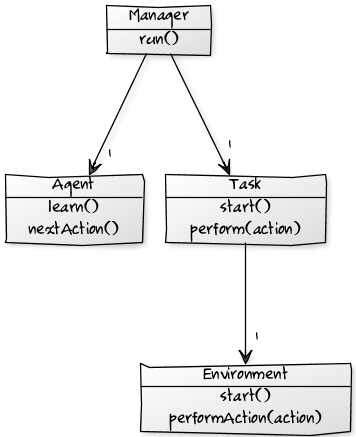
\includegraphics[width=0.5\textwidth]{MCarquitectra.png}
  \caption{Modelo Conceptual Arquitectura.}

\end{figure}
	
	
	\subsection{Uso}
	\subsection{Visualización}
	
\section{Algoritmos de Aprendizaje}
	\subsection{Agentes Model-Free}
		\subsubsection{QLearning}
		\subsubsection{Sarsa}
		\subsubsection{Sarsa ($\lambda$)}	
	\subsection{Agentes Model-Based}	
		\subsubsection{R-max}
		\subsubsection{R-max factorizado}

\section{Ambiente Estocastico}
	\subsection{Resultados}
	



\section{Pruebas y resultados}
	\subsection{Sin Rewards Intermedios}
	\subsection{Rewards Intermedios por posición del bomberman}
	\subsection{Rewards Intermedios por explotar bomba}
	\subsection{Rewards Intermedios por explotar bomba relativo a la posicion de la bomba}

\section{Conclusiones}


	





		


		
		

		
		
		
		
\newpage
\tableofcontents
\newpage
	 
	
\end{document}